%\documentclass[article]{jss}
\documentclass[article,a4paper,nojss,notitle]{jss}
%\providecommand{\IridiaTrCover}[1][]{}
\usepackage{IridiaTrCover}
\newcommand{\techrep}{2011-004}
\newcommand{\techdate}{February 2011}
\newcommand{\revdate}{February 2012}
\newcommand{\revhistory}{%
 2011-004.001 & February 2011\\
 2011-004.002 & February 2012\\
}
\newcommand{\ifIridiaTrElse}[2]{#1}
\newcommand{\IridiaTrOnly}[1]{#1}

\usepackage{algorithm,algorithmic}
\usepackage{booktabs}
\usepackage{tabularx}
\usepackage{xspace}
\usepackage{amsmath,amssymb}
\usepackage{relsize}
\usepackage{fancyvrb}
%%%%%%%%%%%%%%%%%%%%%%%%%%%%%%
%% declarations for jss.cls %%%%%%%%%%%%%%%%%%%%%%%%%%%%%%%%%%%%%%%%%%
%%%%%%%%%%%%%%%%%%%%%%%%%%%%%%
% \newcommand{\true}{\textsc{true}}
% \newcommand{\false}{\textsc{false}}
% \newcommand{\NULL}{\textsc{null}}
\newcommand{\assign}{\ensuremath{:=}}
\newcommand{\procedure}[1]{\textsf{#1}}
\newcommand{\ie}{i.e.}% id est  --       that is
\newcommand{\eg}{e.g.}% exempli gratia -- for example
\newcommand{\etal}{et al.}% et alii -- and others
\newcommand{\mcol}{\multicolumn}
\newcommand{\cmnt}[1]{\footnote{\noindent\textbf{[ #1 ]}}}
\newcommand{\MANUEL}[1]{{\footnotesize\noindent\textbf{[~MANUEL: #1~]}}}
\newcommand{\THOMAS}[1]{\footnote{\noindent\textbf{[ THOMAS: #1 ]}}}
\newcommand{\hide}[1]{}
\newcommand{\iter}{\ensuremath{j}\xspace}
\newcommand{\Budget}{\ensuremath{B}\xspace}
\newcommand{\Budgetj}{\ensuremath{\Budget_{\iter}}\xspace}
\newcommand{\Bused}{\ensuremath{\Budget_\text{used}}\xspace}
\newcommand{\Ncand}[1][]{\ensuremath{N_{#1}}\xspace}
\newcommand{\Mui}{\ensuremath{\mu_{\iter}}\xspace}
%\newcommand{\Nparam}{\ensuremath{{N^\text{param}}}\xspace}
\newcommand{\Nparam}{\ensuremath{{N^\text{param}}}\xspace}
\newcommand{\Niter}{\ensuremath{N^\text{iter}}\xspace}
\newcommand{\tEstimate}{\ensuremath{\hat{t}}\xspace}
\newcommand{\Nmin}{\ensuremath{N^\text{min}}\xspace}
\newcommand{\Nsurv}{\ensuremath{N^\text{surv}}\xspace}
\newcommand{\Nelite}{\ensuremath{N^\text{elite}}\xspace}
\newcommand{\Nnew}{\ensuremath{N^\text{new}}\xspace}
\newcommand{\Celite}{\ensuremath{\Theta^\text{elite}}\xspace}
\newcommand{\cparent}{\ensuremath{\theta^\text{parent}}\xspace}

\newcommand{\irace}{\pkg{irace}\xspace}
\newcommand{\race}{\pkg{race}\xspace}
\newcommand{\FRACE}{\text{F-Race}\xspace}
\newcommand{\IFRACE}{\text{I/F-Race}\xspace}
\newcommand{\aR}{\proglang{R}\xspace}
\newcommand{\iraceversion}{1.0}
\newcommand{\pvalue}{$p$~value\xspace}
\newcommand{\ttest}{$t$~test\xspace}

\newcommand{\parameter}[1]{\code{#1}}
\renewcommand{\enspace}{}

\newcommand{\SoftwarePackage}{\pkg}
\newcommand{\ACOTSP}{\SoftwarePackage{ACOTSP}\xspace}
\newcommand{\SPEAR}{\SoftwarePackage{SPEAR}\xspace}



%\ifIridiaTrElse{%
% \author{
%   \begin{minipage}[c]{0.9\linewidth}
%     \begin{center}
%       \begin{tabular*}{0.7\linewidth}{@{\extracolsep{\fill}}lr}
%         Manuel L\'opez-Ib\'a\~nez &\email{manuel.lopez-ibanez}{ulb.ac.be} \\    
%         J\'er\'emie Dubois-Lacoste & \email{jeremie.dubois-lacoste}{ulb.ac.be} \\               
%         Thomas St\"utzle & \email{stuetzle}{ulb.ac.be} \\              
%         Mauro Birattari & \email{mbiro}{ulb.ac.be} \\                 
%       \end{tabular*}\\[1.5ex]
%      \normalsize\emph{IRIDIA, CoDE, Universit\'e Libre de Bruxelles, Brussels, Belgium}\\
%       Contact: \email{irace}{iridia.ulb.ac.be}
%     \end{center}
%   \end{minipage}}
% }
\date{\revdate}
% }{%
% %% almost as usual
\author{Manuel L\'opez-Ib\'a\~nez, J\'er\'emie Dubois-Lacoste,
  Thomas St\"utzle and        Mauro Birattari
\\IRIDIA, CoDE, Universit\'e Libre de Bruxelles, Brussels, Belgium}

\title{The \irace Package:\\ Iterated Racing for\\ Automatic Algorithm Configuration}

% %% for pretty printing and a nice hypersummary also set:
\Plainauthor{Manuel L\'opez-Ib\'a\~nez, J\'er\'emie Dubois-Lacoste, Thomas St\"utzle, Mauro Birattari} %% comma-separated
\Plaintitle{The irace Package: Iterated Race for Automatic Algorithm Configuration} %% without formatting
%\Shorttitle{A Capitalized Title} %% a short title (if necessary)


%% an abstract and keywords
\Abstract{ The \irace package implements the \emph{iterated racing}
  procedure, which is an extension of Iterated F-race 
  (\IFRACE).  The main use of \irace is the automatic configuration of
  optimization algorithms, that is, finding the most appropriate
  settings of an optimization algorithm given a set of instances of an
  optimization problem. It builds upon the \pkg{race} package by
  Birattari and it is implemented in \aR. This paper describes \irace
  version \iraceversion. The \irace package is available from CRAN.
  More information about \irace is available at 
  \url{http://iridia.ulb.ac.be/irace}.}
%
\Keywords{automatic
  algorithm configuration, racing, parameter tuning, \aR}
%
\Plainkeywords{automatic algorithm configuration, racing, parameter
  tuning, R} %% without formatting
%% at least one keyword must be supplied

% %% publication information
% %% NOTE: Typically, this can be left commented and will be filled out by the technical editor
% %% \Volume{13}
% %% \Issue{9}
% %% \Month{September}
% %% \Year{2004}
% %% \Submitdate{2004-09-29}
% %% \Acceptdate{2004-09-29}

%% The address of (at least) one author should be given
%% in the following format:
\Address{
  Manuel L\'opez-Ib\'a\~nez, J\'er\'emie Dubois-Lacoste,
  Thomas St\"utzle, Mauro Birattari  \\    
  IRIDIA, CoDE,\\
  Universit\'e Libre de Bruxelles (ULB)\\
  1050 Brussels, Belgium\\

  E-mail: 
\begin{align*}
  &\email{manuel.lopez-ibanez@ulb.ac.be}\\
  &\email{jeremie.dubois-lacoste@ulb.ac.be}\\
  &\email{stuetzle@ulb.ac.be}\\
  &\email{mbiro@ulb.ac.be}\\
\end{align*}
%   URL: 
% \begin{align*}
%   &\text{\url{http://iridia.ulb.ac.be/~manuel}}\\
%   &\text{\url{http://iridia.ulb.ac.be/~jdubois}}\\
%   &\text{\url{http://iridia.ulb.ac.be/~stuetzle}}\\
%   &\text{\url{http://iridia.ulb.ac.be/~mbiro}}\\
% \end{align*}
\\
\\
}
%% It is also possible to add a telephone and fax number
%% before the e-mail in the following format:
%% Telephone: +43/1/31336-5053
%% Fax: +43/1/31336-734

%% for those who use Sweave please include the following line (with % symbols):
%% need no \usepackage{Sweave.sty}

%% end of declarations %%%%%%%%%%%%%%%%%%%%%%%%%%%%%%%%%%%%%%%%%%%%%%%

\begin{document}
\IridiaTrCover[%
   author={%
 Manuel \textsc{L\'opez-Ib\'a\~nez} \and J\'er\'emie \textsc{Dubois-Lacoste}%
 \and Thomas \textsc{St\"utzle} \and Mauro \textsc{Birattari}
 },
   date=\techdate,
   number=\techrep,
   revdate=\revdate,
   history=\revhistory]

\maketitle

%% include your article here, just as usual
%% Note that you should use the \pkg{}, \proglang{} and \code{} commands.

% Capitalization in sentence style
\section{Introduction}

The  \irace package implements the \emph{iterated racing} procedure,
which is an extension of Iterated F-race  (\IFRACE)
proposed by \citet{BalBirStu07} and further developed by
\citet{BirYuaBal2010:emaoa}. \irace is implemented as an 
\aR package~\citep{Rmanual} and it builds upon the \pkg{race} package by
\citet{IRIDIA-2003-037}.
%
The main purpose of \irace is to automatically configure optimization
algorithms by finding the most appropriate settings given a set of
tuning instances of an optimization problem. For example, tuning a
computer program for logistic routing of trucks such that 
cost is minimized. Nonetheless, automatic configuration methods are
also applicable to any %computer
system that has a number of configurable parameters, and whose
performance on a particular problem often depends on the particular
settings of these parameters. An example could be the tuning of an
industrial process.
%is the tuning of optimization
% passes in source-code compilers, where performance is often evaluated
% by compiling a benchmark set of programs using a particular
% configuration of the compiler, and measuring the running time of the
% executable programs. Another example is the setup of database
% management systems, which may be finely tuned by setting various
% parameters, and where performance is measured in terms of the time
% required by various operations, such as queries, updates, etc. 

We are particularly interested in the tuning of metaheuristics, that
is, general-purpose optimization algorithms such as evolutionary
algorithms~\citep{Goldberg89}, ant colony
optimization~\citep{DorStu2004:book}, and other stochastic local
search methods~\citep{HooStu05sls-mk}. Automatic
configuration methods may also be used for designing complex
algorithms, by finding a particular configuration of a framework
composed by alternative design choices and complementary algorithmic
components~\citep{KhuXuHooLey2009:satenstein,LopStu2012tec}.

The scenario that \irace addresses is usually described as
\emph{offline configuration}~\citep{Birattari09tuning}, that is, there
are two clearly delimited phases. In a primary tuning phase, an
algorithm configuration is chosen, given a set of tuning instances
representative of a particular problem. In a secondary production (or
testing) phase, the chosen algorithm configuration is used to solve
unseen instances of the same problem. The goal is to find, during the
tuning phase, an algorithm configuration that minimizes some cost
measure over the set of instances that will be seen during the
production phase. In other words, the ultimate purpose is that the high-quality
configuration of the algorithm found during the tuning phase
generalizes to similar but unseen instances.

Offline configuration is frequently performed ad-hoc by algorithm designers
as a result of trial-and-error runs of candidate algorithms they
consider. Computational methods for offline configuration involve the use of
experimental design
techniques~\citep{CoyGolRunWas2001,AdeLag06tuning}, evolutionary
algorithms~\citep{NanEib2006gecco,AnsSelTie2009cp}, local
search~\citep{HutHooLeyStu2009jair} or regression
models~\citep{HutHooLey2011lion}. Another notable example is
sequential parameter optimization (SPO)~\citep{Bar2006newexp}, and the
associated \pkg{SPOT}
package~\citep{BarLasPre2010emaoa,R:SPOT}. \pkg{SPOT} uses statistical
models for finding optimal parameters of optimization algorithms. The
main differences between \pkg{SPOT} and \irace are that the former is
more oriented towards analyzing the impact and interactions of
parameters when applying an algorithm to a single instance or
function, whereas the goal of \irace is to find parameter
configurations that perform well over a large set of instances.


\citet{BirStuPaqVar02:gecco,Birattari2004PhD,Birattari09tuning}
proposed an automatic configuration approach, \FRACE, based on
\emph{racing}~\citep{MarMoo1997air} and Friedman's non-parametric two-way analysis of
variance by ranks. This proposal was later improved by sampling
configurations from the parameter space, and refining the sampling
distribution by means of repeated applications of \FRACE. The
resulting automatic configuration approach was called Iterated F-race
(\IFRACE)~\citep{BalBirStu07,BirYuaBal2010:emaoa}. Although a formal
description of the \IFRACE procedure is given in the original
publications, no implementation of it has been made publicly
available.  The \irace package implements a general \emph{iterated
  racing} procedure, which includes \IFRACE as a special case. It also
implements several extensions already described by
\citet{Birattari2004PhD,Birattari09tuning}, such as the use of the
paired \ttest instead of Friedman's test. We have also added several
original contributions, such as
% the possibility of tuning algorithms for decision problems, where
% the goal is to minimize the computation time, and
a new soft-restart mechanism that prevents premature convergence.


The \irace package presented here has already been extensively tested
in several research
projects. \citet{DubLopStu2011amai,DubLopStu2011cor} used \irace for
tuning the parameters of several iterated greedy (IG) variants for
various objectives in the permutation flow-shop problem (PFSP),
outperforming the state-of-the-art.  \citet{LopStu2010:ants}
automatically configured a flexible ant colony optimization framework
for the bi-objective travelling salesman problem
(bTSP). \citet{MonAydStu2011soco} designed an incremental particle
swarm optimization algorithm for large-scale continuous optimization
problems by means of automatic configuration. \FRACE, the precursor of
\IFRACE, was used to configure an algorithm for the timetabling
competition~\citep{ChiBirSocRos2006jos}. Other automatic configuration
methods have been used in the literature to configure new
state-of-the-art algorithms. For example,
FocusedILS~\citep{HutHooLeyStu2009jair} was used to automatically
configure a highly parameterized tree
search~\citep{HutBabHooHu2007fmcad}, and a framework of SAT
solvers~\citep{KhuXuHooLey2009:satenstein} that won several prizes in
the International SAT competition; as well as tuning the commercial
mixed-integer programming solver CPLEX, and obtaining a significant
speedup over the default settings~\citep{HutHooLey2010:cpaior}.
% Lopez-Ibanez \& Blum configured beam-aco for the TSPTW.  Paola,
% MarcoMontes, TP+PLS, Saifulla, Franco,\footnote{MANUEL: I will
%   update these references last.}
%
These examples demonstrate the potential of automatic configuration of
algorithms, and the profound impact it will have on the way
optimization algorithms are designed and evaluated in the future.
%\MANUEL{More references?}

%\section{Automatic configuration and I/F-race}\label{sec:prelim}
\section{Automatic configuration}\label{sec:prelim}

\subsection{Configurable Algorithms}

Many algorithms for computationally hard optimization problems are
configurable, that is, they have a number of parameters that may be
set by the user. As an example, evolutionary algorithms
(EAs)~\citep{Goldberg89} often require the user to specify settings
like the mutation rate, the recombination operator and the population
size. Another example is CPLEX, a mixed-integer programming solver,
that has more than $76$ configurable parameters affecting the main
algorithm used internally by CPLEX, \eg{}, one can select among
different branching strategies.

The reason these parameters are configurable is that there is no 
single optimal setting for every possible application of the algorithm,
and, in fact, the optimal setting of these parameters depends on the
problem being tackled~\citep{AdeLag06tuning,Birattari09tuning}.

There are two main classes of parameters: \emph{categorical} and
\emph{numerical} parameters. Categorical parameters represent discrete
values without any implicit order or sensible distance measure. An
example is the different recombination operators in EAs.  Numerical
parameters have an implicit order of their values. Examples are the
population size and the mutation rate in EAs. There are also seemingly
categorical parameters but with an implicit order %or distance measure
of their values. An example would be a parameter with three values
$\{$\code{low}, \code{medium}, \code{high}$\}$. Such parameters are
called \emph{ordinal}, and we handle them as numerical
parameters. Finally, parameters may be \emph{subordinate} to other
parameters, that is, they are only relevant for particular values of
other parameters. For example, in a genetic algorithm there may be a
parameter that defines the selection operator. % Each selection operator
%may have specific parameters, which are subordinate to each possible
%value of the selection operator. 
More concretely, the selection operator
could take the values \texttt{roulette\_wheel} or \texttt{tournament}. The value \texttt{roulette\_wheel}  does not have
any specific additional parameters, whereas the value \texttt{tournament}  requires to
specify the value of parameter ``tournament size''. In this case, the parameter ``tournament size'' is subordinate to the fact that the selection operator takes the value \texttt{tournament}.
%let us assume
%a complex algorithm where there are several choices for a hypothetical
%local search parameter, and one of them is simulated annealing. The
%temperature parameter, which is only relevant for simulated annealing,
%only has an effect when the parameter ``local search'' has the value
%``simulated annealing'', and hence, the temperature parameter is a
%subordinate parameter.  
Subordinate parameters are not the same as
constraints on the values of parameters.  For example, given
parameters $a$ and $b$, a constraint may be that $a < b$. Such
constraints limit the range of values that a certain parameter can
take in dependence of other parameters, whereas subordinate parameters
are either disabled or they have a value according to a predefined
range. In some cases, parameter constraints may be modeled by
replacing one of the parameters by a surrogate parameter, \eg{}, $a'
\in (0,1)$, such that $ a = a' \cdot b$.

\subsection{The algorithm configuration problem}\label{sec:algoconf}

%\MANUEL{Discuss the difference between algorithm and implementation?}
In the following, we briefly introduce the algorithm configuration
problem, a formal definition is given by \citet{Birattari09tuning}. 
%
Let us assume that we have a parametrized algorithm with $\Nparam$
parameters, $X_d$, $d=1,\dotsc,\Nparam$, and each of them may take
different values (settings).
%$X_d = \{x_d\}$. 
A configuration of the algorithm $\theta=\{x_1,\dotsc,x_\Nparam\}$ is a unique assignment of
values to parameters, and $\Theta$
denotes the possibly infinite set of all configurations of the
algorithm.

When considering a problem to be solved by this parametrized
algorithm, the set of possible instances of the problem may be seen as
a random variable $\mathcal{I}$ from which instances to be solved are
sampled. We are also given a cost measure $\mathcal{C}(\theta, i)$
that assigns a value to each configuration when applied to a single
problem instance $i$, which is a realization of $\mathcal{I}$.
%$\mathcal{C}\colon \Theta \times \mathcal{I} \to \mathbb{R}$,
% where $\mathcal{C}(\theta, i)$
%measures the cost of configuration $\theta \in \Theta$ on instance
%$i \in \mathcal{I}$. 
Since the algorithm may be stochastic, this cost
measure is often a random variable and the value $c(\theta, i)$ is a
realization of the random variable $\mathcal{C}(\theta, i)$. The cost
value may be the best objective function value found within a given
computation time, or, perhaps, the deviation from the optimum value if
the latter is known. In the case of decision problems, it may
correspond to the computation time required to reach a decision, possibly
bounded by a maximum cut-off time. In any case, the cost measure
assigns a cost value to one run of a particular configuration on a
particular instance. The criterion that we want to optimize when
configuring an algorithm for a problem is a function $c_\theta$ of the cost of a
configuration $\theta$ with respect to the distribution of the random variable $\mathcal{I}$. 
%In that sense, it is a
%statistical parameter  defined on the conditional
%distribution $\mathcal{C}(\theta) = \mathcal{C}(\mathcal{I} \mid
%\theta)$. 
The goal of automatic configuration is finding the best configuration
$\theta^*$ that minimizes $c_\theta$.
%
%\begin{equation}\label{eq:autoconf}
% \theta^* = \arg\min_{\theta \in \Theta} c_\theta\enspace. 
%\end{equation}

A usual definition of $c_\theta$ is %$E[\mathcal{C}(\theta)]$,
the expected cost of $\theta$. The definition of $c_\theta$
determines how to rank the configurations over a set of instances. If
the cost values over different instances are incommensurable, the
median or the sum of ranks may be more meaningful. The precise value
of $c_\theta$ is generally unknown, and it can only be estimated by
sampling. % from $\mathcal{C}(\theta, i)$. 
This sampling is performed in
practice by obtaining realizations $c(\theta, i)$ of the random
variable $\mathcal{C}(\theta, i)$. In other words, by evaluating an
algorithm configuration on instances sampled from $\mathcal{I}$.
% 
Since most algorithms of practical interest are sufficiently complex
to preclude an analytical approach, the configuration of such
algorithms follows an experimental approach, where each experiment is
a run of an implementation of the algorithm under specific experimental
conditions~\citep{Bar2006newexp}.
%
% than the one given
%above. 
%For brevity, we have restricted ourselves to a simpler
%definition that is sufficient for our purposes.


\section{Iterated racing}\label{sec:iterated_racing}

\subsection{An overview of iterated racing} % Iterated F-race (I/F-race)}

The \irace package that we propose in this paper is an implementation
of iterated racing, of which
\IFRACE~\citep{BalBirStu07,BirYuaBal2010:emaoa} is a special case that
uses the Friedman's non-parametric two-way analysis of variance by
ranks.

Iterated racing is a method for
automatic configuration that consists of three steps: (1) sampling new
configurations according to a particular distribution, (2) selecting
the best configurations from the newly sampled ones by means of
racing, and (3) updating the sampling distribution in order to bias
the sampling towards the best configurations. These three steps are
repeated until a termination criterion is met.

In iterated racing, each configurable parameter has an independent
sampling distribution, which is either a normal distribution for
numerical parameters, or a discrete distribution for categorical
parameters. The update of the distributions consists of modifying the
sampling distributions, the mean and standard deviation in the case of
the normal distribution, or the discrete probability values of the
discrete distributions. The update biases the distributions to
increase the probability of sampling, in future iterations, the
parameter values in the best configurations found.

After new configurations are sampled, the best configurations are
selected by means of racing. Racing was first proposed in machine
learning to deal with the problem of model
selection~\citep{MarMoo1997air}.  \citet{BirStuPaqVar02:gecco} adapted
the procedure for the configuration of optimization algorithms. A race
starts with a finite set of candidate  configurations. At
each step of the race, the candidate configurations are evaluated on a
single instance. After each step, those candidate configurations that
perform statistically worse than at least another one are discarded,
and the race continues with the remaining \emph{surviving}
configurations. This procedure continues until reaching a minimum
number of surviving configurations, a maximum number of instances that
have been used or a pre-defined computational budget. This
computational budget may be an overall computation time or a number of
experiments, where an experiment is the application of a
configuration to an instance.

The next subsection gives a complete description of the iterated
racing algorithm as implemented in the \irace package. We mostly
follow the description of the original
papers~\citep{BalBirStu07,BirYuaBal2010:emaoa}, adding some details
that were not explicitly given there. Later in
Section~\ref{sec:extensions}, we mention several extensions that were
not proposed in the original publications.

% The racing approach is particularly suited for identifying the best
% configuration from a given initial set of configurations. This initial
% set may  be generated by randomly sampling the parameter space,
% however, in this case, the number of configurations must be large
% enough to sample with a significant probability at least one
% high-performing configuration. In most cases, the parameter space is
% too large, and sampling it effectively would require an excessive
% number of initial configurations.



% \IFRACE was proposed~\citep{BalBirStu07,BirYuaBal2010:emaoa} as an
% extension of \FRACE in order to search the configuration space more
% effectively by focusing on the most promising configurations. \IFRACE
% repeatedly applies \FRACE, and the candidate configurations
% evaluated in each subsequent race depend on the results of the previous
% races. Candidate configurations are generated by sampling according to
% some probability distribution $P_X$ defined over the parameter space
% $X$. Without prior knowledge, the sampling is initially done according
% to a uniform distribution. In subsequent iterations, numerical
% parameters are sampled according to a normal distribution, whereas
% categorical parameters are sampled according to a discrete probability
%function. 

%\subsection{Racing}



\subsection[The iterated racing algorithm in the irace package]{The iterated racing algorithm in the \irace package}\label{sec:irace}

In this section, we describe the implementation of iterated racing as
proposed in the \irace package. The setup of the \irace package itself
is given in Section~\ref{sec:setup}.

An outline of the iterated racing algorithm is given in
Algorithm~\ref{alg:irace}. Iterated racing requires as input: a set of
instances $I$ sampled from $\mathcal{I}$, a parameter space ($X$), a
cost function ($\mathcal{C}$), and a tuning budget ($\Budget$).

\begin{algorithm}[tb]
\caption{Iterated Racing}\label{alg:irace}
\begin{algorithmic}[1]
\REQUIRE $I = \{I_1,I_2,\dotsc\} \sim\mathcal{I}$,\newline
parameter space: $X$,\newline
cost measure: %$\mathcal{C}\colon \Theta
%\times \mathcal{I} \to \mathbb{R}$
$\mathcal{C}(\theta, i) \in \mathbb{R}$,\newline
tuning budget: $\Budget$
\STATE $\Theta_1 \sim \procedure{SampleUniform}(X)$
\STATE $\Celite \assign \procedure{Race}$($\Theta_1$, $\Budget_1$)
  \STATE $j \assign 2$
\WHILE{$\Bused \leq \Budget$}
  \STATE $\Theta^\text{new} \sim \textsf{Sample}(X, \Celite)$
\STATE $\Theta_j \assign \Theta^\text{new} \cup \Celite$
\STATE $\Celite \assign \procedure{Race}$($\Theta_j$, $\Budgetj$)
\STATE $\iter \assign j + 1$
% \IF{$j > \Niter$}
% \STATE $\Niter \assign j$
% \ENDIF
\ENDWHILE
\STATE \textbf{Output:} $\Celite$
\end{algorithmic}
\end{algorithm}

% \begin{algorithm}[tb]
% \caption{\procedure{Race}($\Theta_{\iter}$, $\Budgeti$)}\label{alg:race}
% \begin{algorithmic}[1]
% \STATE $s \assign 1$
% \REPEAT
% \FOR{$\theta_k \in \Theta_{\iter}$}
% \STATE $\Celite \assign \procedure{Race}$($\Theta_1$, $\Budget_1$)
% \STATE $\Nsurv \assign |\Theta_{\iter}|$
% \ENDFOR
% \UNTIL{$\Budgeti < \Nsurv$ \textbf{or} $\Nsurv \leq \Nmin$}
% \STATE \textbf{Output:} $\Celite$
% \end{algorithmic}
% \end{algorithm}

Iterated racing requires an estimation of the number of iterations
$\Niter$ (races) that it will execute. The default setting of $\Niter$
depends on the number of parameters with $\Niter = \lfloor 2 +
\log_{2}\Nparam \rfloor$. Each iteration performs one race with a
limited computation budget $\Budgetj = (\Budget - \Bused) / (\Niter -
\iter + 1)$, where $\iter = 1, \dotsc, \Niter$. Each race starts from
a set of candidate configurations $\Theta_\iter$. The number of
candidate configurations is calculated as $|\Theta_\iter|=
\Ncand[\iter] = \lfloor \Budgetj / (\mu + \min(5,\iter))\rfloor$.
Thus, the number of candidate configurations decreases with the number
of iterations, which means that more evaluations per configuration
will be performed in later iterations. The parameter $\mu$ allows the
user to influence the ratio between budget and number of
configurations, which also depends on the iteration number
$\iter$. The idea behind this setting is that configurations generated in
later iterations will be more similar, and, hence, more evaluations
will be necessary to identify the best ones. On the other hand, we do
not consider for computing this setting more than five iterations, in
order to avoid having too few configurations in a single race.

\newcommand{\Tfirst}{\ensuremath{T^\text{first}}\xspace}
\newcommand{\Teach}{\ensuremath{T^\text{each}}\xspace}

In the first iteration, the initial set of candidate configurations is
generated by uniformly sampling the parameter space $X$. When a race
starts, each configuration is evaluated on the first instance by means
of the cost measure $\mathcal{C}$. Configurations are iteratively
evaluated on subsequent instances until a number of instances have
been seen ($\Tfirst$). Then, a statistical test is performed on the
results. If there is enough statistical evidence to identify some
candidate configurations as performing worse than at least another
configuration, the worst configurations are removed from the race,
while the others, the \emph{surviving} candidates, are run on the next
instance.

There are several alternatives for selecting which configurations
should be discarded during the race. The \FRACE
algorithm~\citep{BirStuPaqVar02:gecco,Birattari09tuning} relies on the
non-parametric Friedman's two-way analysis of variance by ranks, the
Friedman test, and its associated post-hoc test, as described by
Conover~\citep{Conover99:pns}. Nonetheless, the \pkg{race}
package~\citep{IRIDIA-2003-037} implements various alternatives based
on the paired \ttest with and without \pvalue correction for multiple
comparisons, which are also available in the proposed \irace
package.

A new statistical test is performed every $\Teach$ instances. By
default $\Teach=1$, but in some situations it may be helpful to only
perform each test after the configurations have been evaluated on a
number of instances.  The race continues until the budget of the
current iteration is not enough to test all remaining candidate
configurations on a new instance ($\Budgetj < \Nsurv_{\iter}$), or when at
most $\Nmin$ configurations remain, $\Nsurv_{\iter} \leq \Nmin$.
%The value of $\Nmin$ may be specified using
%option \parameter{minNbSurvival}, and the current default is $\Nmin =
%\lfloor 2 + \log_2\Nparam\rfloor$.



At the end of a race, the surviving configurations are assigned a rank
$r_z$ according to the sum of ranks or the mean cost, depending on
which statistical test is used during the race. The $\Nelite_{\iter} =
\min(\Nsurv_{\iter}, \Nmin)$ configurations with the lowest rank are selected
as the set of elite configurations $\Celite$.

In the next iteration, before a race, a number of $\Nnew_{\iter} = \Ncand[\iter] - \Nelite_{\iter-1}$ new
candidate configurations are generated. For generating a new
configuration, first one parent configuration $\theta_z$ is
sampled from the set of elite configurations $\Celite$
with a probability:
%
\begin{equation}\label{eq:weight}
  p_z = \frac{\Nelite_{\iter-1} - r_z + 1}{\Nelite_{\iter-1} \cdot (\Nelite_{\iter-1} + 1) /2}\enspace,
\end{equation}
%
which is proportional to its rank $r_z$. Hence, higher ranked
configurations have a higher probability of being selected as parents.

Next, a new value is sampled for each parameter $X_d$,
$d=1,\dotsc,\Nparam$, according to a distribution that its associated
to each parameter of $\theta_z$. Parameters are considered in the
order determined by the dependency graph of conditions, that is,
non-subordinate parameters are sampled first, those parameters that are
subordinate to them are sampled next if the condition is satisfied,
and so on. Moreover, if a subordinate parameter that was disabled in
the parent configuration becomes enabled in the new configuration,
then the parameter is sampled uniformly, as in the initialization
phase.

If $X_d$ is a numerical parameter defined within the range $[\underline{x}_d, \overline{x}_d]$, then a new value is sampled from
the truncated normal distribution $\mathcal{N}(x_d^z,\sigma_d^{\iter})$, such that the new value is within
the given range.\footnote{%
  For sampling from a truncated normal distribution, we use the
  \pkg{msm} package~\citep{Jac2011jss}.} The mean of the
distribution $x_d^z$ is the value of parameter $d$ in elite
configuration $\theta_z$. The parameter $\sigma_d^{\iter}$ 
%controlling the standard deviation of the distribution 
is initially set to $(\overline{x}_d
- \underline{x}_d)/ 2$, and it
is decreased at each iteration before sampling:
%
\begin{equation}\label{eq:sigma}
  \sigma_d^{\iter} \assign  \sigma_d^{\iter-1} \cdot \left(\frac{1}{\Nnew_{\iter}}\right)^{1/\Nparam}
\end{equation}
%
By reducing $\sigma_d^{\iter}$ in this manner at each iteration, the sampled
values are increasingly closer to the value of the parent configuration,
 focusing the search around the best parameter settings
found as the iteration counter increases. Roughly speaking, the multi-dimensional volume of the sampling
region is reduced by a constant factor at each iteration, but the
reduction factor is higher when sampling a larger number of new
candidate configurations ($\Nnew_{\iter}$).

If the numerical parameter is of integer type, we round the sampled
value to the nearest integer. The sampling is adjusted to avoid the
bias against the extremes introduced by rounding after sampling from a
truncated  distribution.
% \footnote{We simulate
%   sampling an integer ${1,2,3}$ by sampling a real value $x$ from the truncated normal distribution 
% $D(\text{mean}=2.5, \text{min}=1, \text{max}=4)$,  and then rounding such that:
% \[
% \text{round}(x) = \begin{cases} 
% 1 & \text{if $1 \leq x < 1.5$}\\
% 2 & \text{if $1.5 \leq x < 2.5$}\\
% 3 & \text{if $2.5 \leq x < 3$}\\
% \end{cases}
% \]

% $D(\text{mean}=2, \text{min}=1, \text{max}=3)$,  and then rounding such that:
% \[
% \text{round}(x) = \begin{cases} 
% 1 & \text{if $1 \leq x < 1.5$}\\
% 2 & \text{if $1.5 \leq x < 2.5$}\\
% 3 & \text{if $2.5 \leq x < 3$}\\
% \end{cases}
% \]
% %
% Hence, it is two times less probable (conditioned to the underlying
% sampling distribution $D$) to sample a particular extreme value than a
% particular non-extreme value. We remove this bias by sampling $x$ instead from $D(\text{mean}=2.5, \text{min}=1,\text{max}=4)$ and computing $\text{round}(x-0.5)$.}

If $X_d$ is a categorical parameter with levels $X_d \in \{x_1, x_2,
\dotsc, x_{n_d} \}$, then a new value is sampled from a discrete
probability distribution $\mathcal{P}^{\iter,z}(X_d)$. In the first iteration ($\iter = 1$), $\mathcal{P}^{1,z}(X_d)$ is uniformly distributed over
the domain of $X_d$. In subsequent iterations, it is updated before
sampling as follows:
%
\begin{equation}\label{eq:prob_update}
  \mathcal{P}^{\iter,z} (X_d = x_j) \assign \mathcal{P}^{\iter-1,z} (X_d = x_j)
  \cdot \left(1 - \frac{\iter-1}{\Niter}\right) + \Delta \mathcal{P}
\end{equation}
where 
\begin{equation}\label{eq:2}
  \Delta \mathcal{P} = 
  \begin{cases}
    \dfrac{\iter - 1}{\Niter} & \text{if $x_j = x_z$}\\
    0  & \text{otherwise}\\
  \end{cases}
\end{equation}
%

Finally, the new configurations generated after sampling inherit the
probability distributions from their parents, and a new race is
launched with the union of the new configurations and the elite
configurations.

The algorithm stops if the budget is exhausted ($\Bused > \Budget$) or
if the number of candidate configurations to be evaluated at the start
of an iteration is not greater than the number of elites
($\Ncand[\iter] \leq \Nelite_{\iter-1}$), since in that case no new
configurations would be generated. If the iteration counter $\iter$
reaches the estimated number of iterations $\Niter$ but there is still
enough remaining budget to perform a new race, we simply increase
$\Niter$ and continue the algorithm.



\section{Extensions}\label{sec:extensions}

We have implemented several extensions that were not proposed in the
original publications.

\subsection{Initial configurations}

We can seed the iterated race procedure with a set of initial
configurations. In that case, only enough configurations are sampled
to reach $\Ncand[1]$ in total.
% For how to specify the initial set of configurations, see option \parameter{candidatesFile}.

%  \subsection{Tuning for computation time}\label{sec:time}

% Sometimes the goal is to minimize the computation time required to
% perform a task. For example, in decision problems, the goal is to
% minimize the time that an algorithm takes to reach an answer. In the
% case of complete algorithms that optimally solve an optimization
% problem, the goal is to minimize the time to find the optimal
% solution and prove its optimality. 

% When automatically configuring an algorithm for minimizing computation
% time, it is often preferred to define the tuning budget $\Budget$ as a
% computation time limit, instead of a maximum number of experiments. In
% such a case, the budget of each iteration is computed as $\Budgetj =
% (\Budget - \Bused) / (\tEstimate_{\iter}\cdot(\Niter - \iter + 1))$,
% where $\iter = 1, \dotsc, \Niter$, and $\tEstimate_{\iter}$ is an
% estimate of the computation time required by a single run of the
% algorithm. The initial value of this estimate is provided by the user,
% for example, as a cut-off time after which an algorithm run is stopped
% even if the termination condition has not been reached.  In subsequent iterations,
% $\tEstimate$ is updated by computing the average time used by the
% experiments performed so far.


\subsection{Soft-restart}

Our implementation incorporates a ``soft-restart'' mechanism to avoid
premature convergence. In the original \IFRACE
proposal~\citep{BalBirStu07}, the standard deviation, in the case of
numerical parameters, or the discrete probability of unselected
parameter settings, in the case of categorical ones, decreases at
every iteration. Diversity is introduced by the variability of the
sampled configurations. However, if the tuning converges to a few, very
similar elite configurations in few iterations, the diversity is lost
and newly generated candidate configurations will not be very
different from the ones already tested. Such a premature convergence
wastes the remaining budget on repeatedly evaluating minor variations
of the same configurations, without exploring new alternatives.

We implemented a ``soft-restart'' mechanism that checks for premature
convergence after generating each new set of candidate configurations.  We consider that there is premature
convergence when the ``distance'' between two candidate
configurations is zero. The
distance between two configurations is defined as the maximum distance
between their parameter settings, which is defined as follows:

\begin{itemize}
\item If the parameter is subordinate and disabled in both configurations, the distance is zero;
\item if it is disabled in one configuration but enabled in the other,
  the distance is one;
\item if the parameter is enabled in both configurations (or it is not subordinate), then: 

  \begin{itemize}
  \item in the case of numerical parameters (integral or real), the
    distance is the absolute normalized difference between their
    values;
 % (the values are rounded to the number of decimal digits
 %    specified by the option \parameter{digits}) ;

  \item in the case of ordinal and categorical parameters, the distance
    is one if the values are different and zero otherwise.
  \end{itemize}
\end{itemize}

When premature convergence is detected, a ``soft-restart'' is applied
by partially reinitializing the sampling distribution. This
reinitialization is applied only to the elite configurations that were
used to generate the candidate configurations with zero distance. The
other elite configurations do not suffer from premature convergence,
thus they may still lead to new configurations, whereas reinitializing
their sampling distribution would mean to lose all the knowledge
accumulated on them.

In the case of categorical parameters, the discrete sampling distribution
of elite configuration $z$, $\mathcal{P}^{\iter,z}(X_d)$, is adjusted
by modifying each individual probability value $p \in
\mathcal{P}^{\iter,z}(X_d)$ with respect to the maximum value
$p_\text{max} = \max\{\mathcal{P}^{\iter,z}(X_d)\}$ as follows:
%
\[p \assign \frac{0.9 \cdot p + 0.1 \cdot p_\text{max}}{\sum_{p' \in \mathcal{P}^{\iter,z}(X_d)} 0.9 \cdot p' + 0.1 \cdot p_\text{max}}\enspace.\]
%
For numerical and ordinal parameters, the standard deviation of elite configuration $z$, $\sigma_d^{\iter,z}$, is ``brought back'' two iterations, with a maximum limit of its value in the second iteration, as follows:
\[
  \sigma_d^{\iter,z} \assign \min\left\{ \sigma_d^{\iter,z} / \left(\frac{1}{\Nnew_{\iter}}\right)^{2/\Nparam},\;
\frac{\overline{x}_d
- \underline{x}_d}{2} \cdot \left(\frac{1}{\Nnew_{\iter}}\right)^{1/\Nparam}\right\}
\]

After adjusting the sampling distribution of all affected elite
configurations, the set of candidate configurations that triggered the
soft-restart is discarded and a new set of $\Nnew$ configurations is
sampled from the elite configurations. This procedure is applied at
most once per iteration.

\section[The irace package]{The \irace package}\label{sec:setup}

We provide here a brief summary of the \irace package. The full
documentation is available together with the package.

The scheme in Fig.~\ref{fig:irace-scheme} describes how the different
parts of \irace interact with each other. The program \irace requires
three main inputs:

\begin{enumerate}
\item A description of the parameter space $X$,
%, which is provided by a
%  file \parameter{parameterFile} that describes
  that is, the parameters to configure, their types, ranges and
  constraints. Section~\ref{sec:paramFile} summarizes how to define a
  parameter space in \irace.

\item The set of tuning instances $\{I_1, I_2, \dotsc\}$, which in
  practice is a finite, representative sample of
  $\mathcal{I}$. The particular options for specifying the set of
  tuning instances are given in Section~\ref{sec:instances}.

\item The configuration of \irace itself, which is defined by a number
  of options.
  % These options may be defined in a configuration file or in the
  % command line.
  Table~\ref{tab:options} maps the description of iterated racing in
  the previous section to the configuration options in \irace. The
  complete list of options is available in the software documentation.
\end{enumerate}

In addition, \irace requires a function (or an auxiliary program)
called \parameter{hookRun}, which is responsible of applying a
particular configuration to an instance and returning the
corresponding cost value.

The \irace package is designed to be used either from within \aR, or
from the command-line by means of a wrapper. We illustrate these two
usage modes by means of simple examples in
Section~\ref{sec:applications}.

% An initial set of configurations may be provided by means of an
% optional candidates file (option \parameter{candidatesFile}). The
% evaluation of candidate configurations is performed in two phases by
% means of two auxiliary programs called ``hooks''. \parameter{hookRun}
% applies a particular configuration to an instance. Once all candidate
% have been applied to the current instance, \parameter{hookEvaluate}
% returns their corresponding cost value. These hooks are described in
% Section~\ref{sec:hooks}. The use of auxiliary programs is intuitively
% straightforward in the common case of configuring a
% command-line-driven program. This setup also provides a high level of
% flexibility, since these auxiliary program are completely under the
% control of the user, who may add to them any level of complexity
% desired in the programming language of their choice. Moreover, The
% separation in two distinct phases allows the user to examine and
% operate on all the results from the first phase before invoking the
% second phase.

% A step-by-step guide of setting
% up a new tuning scenario is provided in the full documentation. Here,
% we illustrate the process with a simple example in
% Section~\ref{sec:applications}.

\begin{figure}[p]
  \centering
  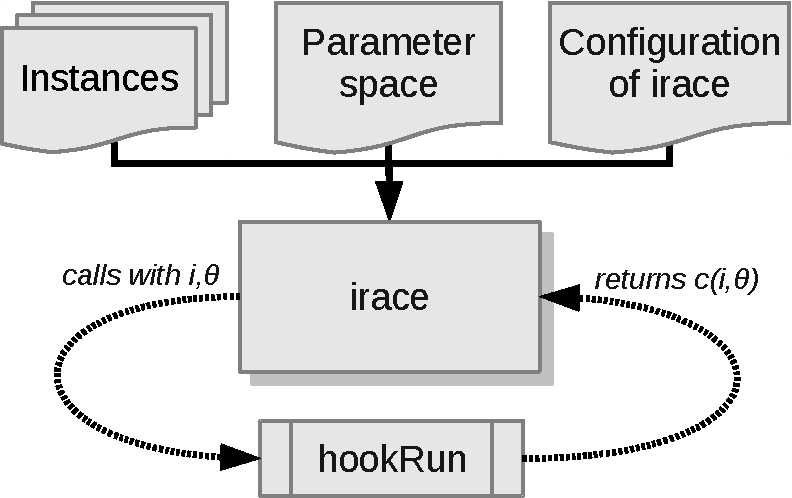
\includegraphics[width=0.6\textwidth]{irace-scheme-simple-crop}
  \caption{Scheme of \irace flow of information.}
\label{fig:irace-scheme}
\end{figure}

\begin{table}[p]
  \centering
  \begin{tabular}[c]{rl}
    \toprule
    \textbf{Iterated racing parameter}&\textbf{\irace configuration option}\\
    \midrule
%    \Budget     & either \parameter{maxNbExperiments} or \parameter{timeBudget}\\
    \Budget     & \parameter{maxExperiments}\\
    $\mathcal{C}$ (cost measure) & \parameter{hookRun}\\ 
% and \parameter{hookEvaluate}, see also Section~\ref{sec:hooks}\\
%    $\Niter$    & \parameter{nbIterations}\\
    $\mu$       & \parameter{mu}\\
    $\Nmin$     & \parameter{minNbSurvival}\\
    \Tfirst     &\parameter{firstTest} \\
    \Teach      & \parameter{eachTest} \\
    Statistical test & \parameter{testType}\\
%    $\tEstimate_1$ & \parameter{timeEstimate}, see also Section~\ref{sec:time}\\
    \bottomrule
  \end{tabular}
  \caption{Configuration options of \irace corresponding to the description of iterated racing given in Section~\ref{sec:irace}. The full list of options is available in the complete documentation.}
  \label{tab:options}
\end{table}

\subsection{Tuning instances}\label{sec:instances}

The set of tuning instances $\{I_1, I_2, \dotsc\}$ may be given
explicitly as a configuration option of \irace. Alternatively, the
instances may be read from an instance file
(\parameter{instanceFile}). The string given by
option \parameter{instanceDir} will be prefixed to them. If the
option \parameter{instanceFile} is not set, then \irace considers all
files found in \parameter{instanceDir}, and recursively in its
subdirectories, as tuning instances. The order in which instances are
considered by \irace is randomized if the
option \parameter{sampleInstances} is enabled. Otherwise, the order is
the same as given in \parameter{instanceFile} if this option is set or
in alphabetical order if there is no \parameter{instanceFile}.

% \subsection{Configuration File}\label{sec:configFile}
 
% The configurable parameters of \irace can be defined in a
% configuration file or on the command-line. The full list of
% configurable parameters is given in
% \autoref{appendixA}. If the same parameter is defined
% both in the configuration file and on the command-line, the value
% given on the command-line has preference. If a parameter is not set
% neither in the configuration file nor on the command-line, the default
% value is used.

\newpage
\subsection{Parameter space}\label{sec:paramFile}

For simplicity, the description of the parameters space is given as a
table. Each line of the table defines a configurable parameter:
%
\begin{Code}
     <name> <label> <type> <range> [ | <condition> ]
\end{Code}
%
where each field is defined as follows:
%
\begin{center}
\renewcommand{\arraystretch}{1.2}
  \begin{tabularx}{0.98\linewidth}{@{}rX}
    \code{<name>} & The name of the parameter as an unquoted
    alphanumeric string,
    for instance: `\code{ants}'.\\
    \code{<label>}& A \emph{label} for this parameter. This is a
    string that will be passed together with the parameter
    to \parameter{hookRun}. In the default \parameter{hookRun}
    provided with the package (Section~\ref{sec:hooks}), this is the
    command-line switch used to pass the value of this parameter, for
    instance `\code{"-{}-ants "}'.\\
    % The value of the parameter is concatenated \emph{without
    % separator} to the switch string when
    % invoking \parameter{hookRun}.\\

    \code &The type of the parameter, either
    \textit{integer},
    \textit{real}, \textit{ordinal} or \textit{categorical}, given as a single letter: `\code{i}', `\code{r}', `\code{o}' or `\code{c}'. \\
    \code &The range or set of values of the parameter.\\
    \code& An optional \emph{condition} that determines
    whether the parameter is enabled or disabled, thus making the
    parameter subordinate. If the condition evaluates to false, then
    no value is assigned to this parameter, and neither the parameter
    value nor the corresponding label are passed
    to \parameter{hookRun}. The condition must be a valid \aR logical
    expression. The condition may contain the name of other parameters
    as long as the dependency graph does not contain any
    cycle. Otherwise, \irace will detect the cycle and stop with an error.\\
  \end{tabularx}
\end{center}

\paragraph{Parameter types and range.}
Parameters can be of four types:
%
\begin{itemize}
\item \textit{Real} parameters are numerical parameters that can take
  any floating-point values within a given range. The range is
  specified as an interval `\code{(<lower bound>,<upper
    bound>)}'. This interval is closed, that is, the parameter value
  may eventually be one of the bounds. The possible values are rounded
  to a number of \emph{decimal places} specified by
  option \parameter{digits}. For example, given the default
  number of digits of $4$, the values $0.12345$ and
  $0.12341$ are both rounded to $0.1234$.
  % However, the values  $0.00001$ and $0.00005$ remain the same.

\item \textit{Integer} parameters are numerical parameters that can
  take only integer values within the given range. The range is
  specified as for real parameters.

\item \textit{Categorical} parameters are defined by a set of possible
  values specified as `\code{(<value 1>, ..., <value n>)}'. The values
  are quoted or unquoted character strings. Empty strings and strings
  containing commas or spaces must be quoted.

\item \emph{Ordinal} parameters are defined by an \emph{ordered} set
  of possible values in the same format as for categorical
  parameters. They are handled internally as integer parameters, where
  the integers correspond to the indexes of the values.

\end{itemize}

Section~\ref{sec:applications} shows examples on how to read the
parameters table either from a string literal or from a file.

% The parameters of the algorithm to be tuned are described in a
% \emph{parameter file}.  These parameters are passed as command-line
% options to the program \parameter{hookRun}. This setup is designed to
% be straightforward for the common case of configuring a
% command-line-driven program. Nonetheless, since \parameter{hookRun} is
% under the control of the user, it may transform its command-line
% parameters into a file and pass this file to another program, or
% perform other more complex steps.


% \paragraph{Subordinate parameters.} 
% A conditional parameter is one that is enabled or disabled depending
% on the values of other parameters. A parameter is marked as
% conditional by adding the character \code{'|'} followed by an \aR
% expression involving the names of other parameters. This expression
% must return \code{TRUE} when the parameter should be enabled, and
% \code{FALSE} otherwise. Examples of operators that are valid in a condition are relational operators 
% (\code{<, >, <=, >=, ==, !=}) and the logical operators: \code{!~\textrm{(not)}, \&\&~\textrm{(logical-and)},
%   ||~\textrm{(logical-or)}}. Another useful operator is
% \code{\%in\%}, which returns \code{TRUE} if its left operand matches any
% element of its right operand. See the example below.

\subsection{hookRun}\label{sec:hooks}

The evaluation of a candidate configuration is done by means of a user-given function or, alternatively, a user-given auxiliary program. The function (or program name) is specified by the option \parameter{hookRun}. 

When \parameter{hookRun} is an \aR function, then it is invoked for each candidate configuration as:
%
\begin{center}
  \begin{CodeInput}
    hookRun(instance, candidate, extra.params, config)
  \end{CodeInput}
\end{center}
%
where \code{instance} is a single instance, \code{extra.params} is a
user-defined value associated to this instance, \code{config} is the
configuration of \irace, and \code{candidate} is a list with three
components: \emph{(1)} \code{\$index}, which is a numeric value
identifying this candidate; \emph{(2)} \code{\$values}, which is a
one-row data frame with one column per parameter value; and \emph{(3)}
\code{\$labels}, which is a list of the labels of each parameter. The
function \code{hookRun} must return a numerical value corresponding to
the cost measure of the candidate configuration on the given instance.

When \parameter{hookRun} is an auxiliary executable program, then it
is invoked for each candidate configuration, passing as arguments: the
instance, a numeric identifier, and the command-line parameters of the
candidate configuration. The numeric identifier uniquely identifies a
configuration within a race (but not across the races in a single
iterated race). The command line is constructed by appending to each
parameter label (switch), \emph{without separator}, the value of the
parameter, following the order given in the parameter table. The
program \parameter{hookRun} must print (only) a real number, which
corresponds to the cost measure of the candidate configuration for the
given instance. The working directory of \parameter{hookRun} is set to
the execution directory specified by the
option \parameter{execDir}. This allows the user to execute several
runs of \irace in parallel without the runs interfering with each
other.

% The evaluation of the candidate configurations is done in two
% phases. In the first phase, the program specified by the
% option  is invoked for each candidate
% configuration, passing as arguments: the instance name, a numeric
% identifier, and the command-line parameters of the candidate
% configuration. The numeric identifier uniquely identifies a
% configuration within a race (but not across the races in a single
% iterated race). The command line is constructed by appending to each
% parameter switch, \emph{without separator}, the value of the
% parameter, following the order given in the parameter file. 
% % If the options \parameter{parallel}, \parameter{mpi}
% % or \parameter{sgeCluster} are enabled, the calls
% % to \parameter{hookRun} happen in parallel.
% The program \parameter{hookRun} should not have any output and it
% should exit with a value of zero.  Once all calls
% to \parameter{hookRun} for the current instance have finished, the
% results are evaluated using the program specified by
% option \parameter{hookEvaluate}.

% In this second phase, the program 
% \parameter{hookEvaluate} is invoked for each candidate configuration
% in order of increasing candidate number. The parameters
% of \parameter{hookEvaluate} are the instance name, the numeric
% identifier and the total number of candidate configurations alive at
% this point of the race. The program \parameter{hookEvaluate} must
% print (only) a real number, which corresponds to the cost measure of
% the candidate configuration for the given instance.

% The working directory of these programs is set to the execution
% directory specified by the option \parameter{execDir}. This allows the
% user to execute several runs of \irace in parallel without the runs interfering with each other.

\section{Examples of tuning scenarios}\label{sec:applications}

The next two sections illustrate two different ways of using
\irace. The first example shows how to set up and use the \irace
package by means of \aR programming. The second example shows how to
tune an external program via the command-line options of the \irace
stand-alone program provided with the package.

\subsection[Tuning optim() from R]{Tuning \code{optim()} from \aR}

In this illustrative example, our goal is to tune the parameters of
the simulated annealing algorithm (SANN) provided by the \code{optim()}
function in the \aR \pkg{base} package. In particular, let's say we
are interested in optimizing instances of the following family of
functions:

\begin{equation}
  \label{eq:1}
  f(x) = \lambda \cdot f_\text{Rastrigin} (x) + (1 - \lambda) \cdot f_\text{Rosenbrock}(x)
\end{equation}
%
where $\lambda$ follows a normal distribution $\mathcal{N}(0.9,
0.02)$, and $f_\text{Rastrigin}$ and $f_\text{Rosenbrock}$ are the
well-known Rastrigin and Rosenbrock benchmark functions. We use the implementation of these functions provided by the package \pkg{cmaes} \citep{R:cmaes}. 

\begin{CodeInput}
f_rosenbrock <- function (x) {
  d <- length(x)
  z <- x + 1
  hz <- z[1:(d - 1)]
  tz <- z[2:d]
  s <- sum(100 * (hz^2 - tz)^2 + (hz - 1)^2)
  return(s)
}
f_rastrigin <- function (x) {
  sum(x * x - 10 * cos(2 * pi * x) + 10)
}
\end{CodeInput}

In this scenario, different instances are given by different values of
$\lambda$. Hence, we first generate $200$ instances as follows:

\begin{CodeInput}
weights <- rnorm(200, mean = 0.9, sd = 0.02)
\end{CodeInput}

We are interested in optimizing two parameters of the SANN algorithm: \code{tmax} and \code{temp}. We setup the parameter space as follows:

\begin{CodeInput}
parameters.table <- '
tmax "" i (1, 5000)
temp "" r (0, 100)
'
\end{CodeInput}

and we use the \irace function \code{readParameters} to read this table:

\begin{CodeInput}
R> library("irace")
R> parameters <- readParameters(text=parameters.table)
\end{CodeInput}

Next, we define the function that will evaluate each candidate
configuration on a single instance. For simplicity, we restrict to
three-dimensional functions and we set the maximum number of
iterations of SANN to $5000$.

\begin{CodeInput}
hook.run <- function(instance, candidate, extra.params = NULL, config = list())
{
  D <- 3
  par <- runif(D, min=-1, max=1)
  fn <- function(x) {
    weight <- instance
    return(weight * f_rastrigin(x) + (1 - weight) * f_rosenbrock(x))
  }
  res <- optim(par,fn, method="SANN",
               control=list(maxit=5000
                 , tmax = as.numeric(candidate$values[["tmax"]])
                 , temp = as.numeric(candidate$values[["temp"]])
                 ))
  return(res$value)
}
\end{CodeInput}

We are now ready to launch \irace. We do it by means of the
\code{irace} function by setting \code{hookRun} to the function define
above, \code{instances} to the first $100$ random weights, and a
maximum budget of $1000$ calls to \code{hookRun}.

\begin{CodeChunk}
\begin{CodeInput}
R> result <- irace(tunerConfig = list(
                    hookRun = hook.run,
                    instances = weights[1:100],
                    maxExperiments = 1000),
                  parameters = parameters)
\end{CodeInput}
\end{CodeChunk}

The function \code{irace} will print information about its progress. We can print the best configurations found as follows:

\begin{CodeChunk}
\begin{CodeInput}
R> candidates.print(result)
\end{CodeInput}
\begin{CodeOutput}
      tmax   temp
118 3501 0.8984
126 3487 1.1865
103 3441 0.3150
\end{CodeOutput}
\end{CodeChunk}

We could now evaluate the cost of the best configuration found by
\irace versus the default configuration of SANN on the other $100$
instances previously generated and not used during training.

\begin{CodeChunk}
\begin{CodeInput}
R> default <- sapply(weights[101:200], hook.run,
                  candidate=list(values=list(tmax=10,temp=10)))

R> result.list <- as.list(removeCandidatesMetaData(result[1,]))
R> tuned <- sapply(weights[101:200], hook.run, candidate=list(values=result.list))

R> boxplot(list(default=default, tuned=tuned))
\end{CodeInput}
\end{CodeChunk}      

The resulting plot is given in Fig.~\ref{fig:boxplot_sann}. The
boxplot clearly shows that the tuned configuration is able to find
better solutions than the default configuration of SANN. This small example is included in the documentation of the \irace package and can be run with the command:



\begin{figure}
  \centering
  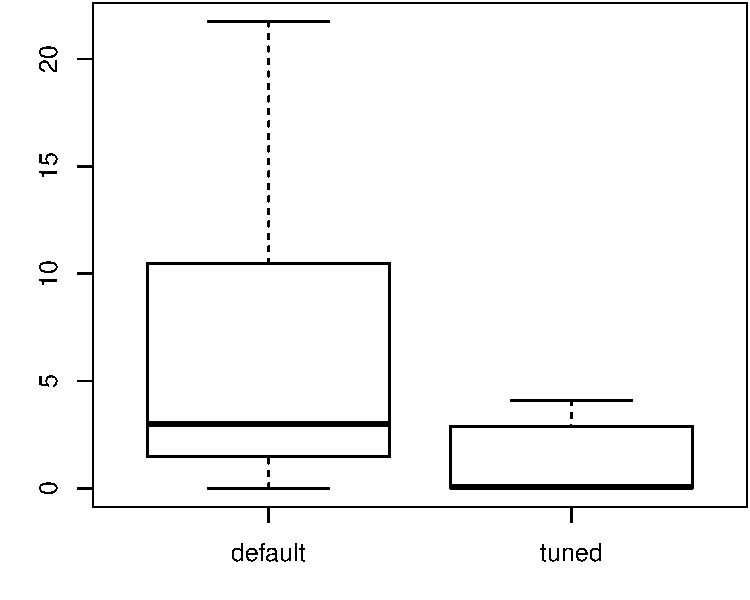
\includegraphics[width=0.5\textwidth]{boxplot-sann.pdf}
  \caption{Boxplot of default vs. tuned configuration of SANN}
  \label{fig:boxplot_sann}
\end{figure}

\begin{CodeChunk}
\begin{CodeInput}
R> example(irace)
\end{CodeInput}
\end{CodeChunk}      


\subsection[Tuning ACOTSP]{Tuning \ACOTSP}

\ACOTSP~\citep{Stu2002} is a software package that implements various
ant optimization algorithms to tackle the symmetric traveling salesman
problem (TSP). The example proposed here concerns the automatic
configuration of all its $11$ parameters.  The goal is to find a
configuration of \ACOTSP that obtains the lowest solution cost in
TSP instances within a given computation time limit. The setup of the
tuning procedure is defined through various files.

\begin{figure}
  \centering
%\begin{Verbatim}[frame=single,framesep=3mm,label=\code{~parameters.txt~}]
\begin{CodeInput}
# name      switch           type values    [| conditions (using R syntax)]
algorithm   "--"             c    (as,mmas,eas,ras,acs)
localsearch "--localsearch " c    (0, 1, 2, 3)
alpha       "--alpha "       r    (0.01, 5.00)
beta        "--beta "        r    (0.01, 10.00)
rho         "--rho  "        r    (0.00, 1.00)
ants        "--ants "        i    (5, 100)
nnls        "--nnls "        i    (5, 50)    | localsearch %in% c(1, 2, 3)
q0          "--q0 "          r    (0.0, 1.0) | algorithm %in% c("acs")
dlb         "--dlb "         c    (0, 1)     | localsearch %in% c(1,2,3)
rasrank     "--rasranks "    i    (1, 100)   | algorithm %in% c("ras")
elitistants "--elitistants " i    (1, 750)   | algorithm %in% c("eas")
\end{CodeInput}
% \end{Verbatim}\vspace{-3ex}
\caption{Parameter file (\code{parameters.txt}) for tuning \ACOTSP.}\label{fig:acotsp_parameters}
\end{figure}

\begin{figure}
  \centering
%\begin{Verbatim}[frame=single,framesep=3mm,label=\code{~tune-conf~}]
\begin{CodeInput}
execDir <- "./tuning/"
maxExperiments <- 1000
\end{CodeInput}
%\end{Verbatim}\vspace{-3ex}
\caption{Configuration file (\code{tune-conf}) for tuning \ACOTSP.}\label{fig:tune_conf}
\end{figure}

First, we define a parameter file (\code{parameters.txt},
Fig.~\ref{fig:acotsp_parameters}) that describes the parameter space.
We also create a configuration file (\code{tune-conf},
Fig.~\ref{fig:tune_conf}) to overwrite some default options of \irace.
In particular, we set an execution directory (e.g., \code{./tuning/})
where temporary files are stored, and we set the tuning budget to
$1\,000$ runs of \ACOTSP. Next, we place the tuning instances in the
subdirectory \code{./Instances/}, which is the default value of the
option \parameter{instanceDir}. We create a basic \code{hook-run}
script that simply runs the \ACOTSP software for 20 seconds and prints
the objective value of the best solution found.\footnote{The package
  includes an example of this \code{hook-run} script for Unix
  environments, which can be found at
  \code{file.path(system.file(package="irace"), "examples","acotsp")}.}
We can now launch the tuning procedure as follows:
  \begin{CodeInput}
R> library("irace")
R> irace.cmdline()
\end{CodeInput}

The package provides a convenient command-line wrapper for Unix
environments, called \code{irace}, located in
\code{file.path(system.file(package="irace"), "bin")}, that basically
invokes \aR and executes the commands above. The command-line wrapper
also allows the user to specify many options directly from the
command-line.

Most of the output is generated by the underlying \race package, which
prints a detailed progress of each race. After each race finishes, the
set of elite configurations are printed. At the end, the best
configurations found are printed as a table and as command-line
parameters:

\begin{footnotesize}
%\begin{verbatim}
\begin{CodeOutput}
# Best candidates
    algorithm localsearch alpha   beta    rho ants nnls     q0 dlb rasrank elitistants
189       acs           3 1.268 6.0930 0.6846   20   17 0.2812   1      NA          NA
332       acs           3 3.100 0.7011 0.4789   55   11 0.2630   1      NA          NA
320      mmas           3 1.361 9.0390 0.6852   64   25     NA   1      NA          NA
# Best candidates (as commandlines)
                                                                                  command
189  --acs --localsearch 3 --alpha 1.268 --beta 6.0930 --rho  0.6846 --ants 20 --nnls 17  \
    --q0 0.2812 --dlb 1
332  --acs --localsearch 3 --alpha 3.100 --beta 0.7011 --rho  0.4789 --ants 55 --nnls 11  \
    --q0 0.2630 --dlb 1
320  --mmas --localsearch 3 --alpha 1.361 --beta 9.0390 --rho  0.6852 --ants 64 --nnls 25 \
    --dlb 1
\end{CodeOutput}
%\end{verbatim}
\end{footnotesize}

In addition, \irace saves an \proglang{R} dataset file, by
default as \code{irace.Rdata}, which may be read from \proglang{R}
by means of the function \code{load()}. This dataset contains a list \code{tunerResults}, whose elements are: 

\begin{itemize}
\item \code{tunerConfig}: the configuration of \irace.
\item \code{parameters}: the parameter space.
\item \code{experiments}: a matrix storing the result of all
  experiments performed across all iterations. Each entry is the
  result of evaluating one configuration on one instance at a
  particular iteration. The first column (`\code{instance}') indicates
  the instance tested in the experiments of the same row.  The second
  column (`\code{iteration}') gives the iteration (race) number in
  which the experiments in the same row where performed. The remainder
  of the columns represent configurations, and their column names
  correspond to their IDs. Finally, `\code{NA}' represents that for some
  reason the candidate was not evaluated on a particular instance at
  that iteration, either because it did not exist yet or it was removed
  earlier.
\item \code{allCandidates}: a data frame with all candidate
  configurations tested during the execution of \irace.
\end{itemize}


% \subsection[Tuning SPEAR for computation time]{Tuning \SPEAR for computation time}

% \SPEAR~\citep{HutBabHooHu2007fmcad} is a state-of-the-art theorem prover for
% solving industrial SAT instances. It is highly configurable, with a
% total of $26$ parameters, including continuous, integer and
% categorical parameters. For this reason,
% \citet{HutHooStu07aaai} and \citet{HutHooLeyStu2009jair} have
% used it extensively as a benchmark for testing automatic tuning tools.

% We consider in this section the tuning of \SPEAR as a case study of
% using \irace for tuning algorithms for decision problems.  We are only
% interested in how much time is required by \SPEAR to decide whether a
% given SAT instance is satisfiable. \SPEAR stops after a given cut-off
% time if it cannot determine an answer. Therefore, the computation
% effort of the tuning is given by the total computation time consumed
% by \SPEAR. We assign a total time budget (option \parameter{timeBudget}) of 2.4 hours ($8\,640$ seconds). In
% order to calculate the number of experiments that may be performed in
% the remaining budget, we need an estimate of the time required by a
% single run of \SPEAR. In the first iteration of \irace, this estimate
% needs to be provided by the user (option \parameter{timeEstimate}). As
% a worst-case estimate, we set this option to the same value as the
% cut-off time of \SPEAR, which we set to 10 seconds in this example. In
% subsequent iterations, the estimate is adjusted automatically by
% \irace. We also decided to use a \ttest instead of the default
% Friedman-test, because we have some prior knowledge that the \ttest
% produces better results in this setup. The \irace configuration file
% (\code{tune-conf}) for this setup is given in
% Fig.~\ref{fig:tune_conf_spear}. Examples of parameter file and hooks
% for this setup are provided in the examples accompanying the \irace
% package, and the tuning is launched as in the previous example.

% \begin{figure}
%   \centering
% %\begin{Verbatim}[frame=single,framesep=3mm,label=\code{~tune-conf~}]
% \begin{CodeInput}
% execDir <- "./tuning/"
% timeBudget <- 8640
% timeEstimate <- 10
% testType <- "t-test"
% \end{CodeInput}
% %\end{Verbatim}\vspace{-3ex}
% \caption{Configuration file (\code{tune-conf}) for tuning \SPEAR.}\label{fig:tune_conf_spear}
% \end{figure}

%  This setup is summarized in
% Table~\ref{tab:spear_tuning_conf}.  In our experiments, we use a
% benchmark set of software verification instances~\cite{BabHu2007cav},
% with 302 training instances and 302 test instances.

% \begin{table}[th]
%   \centering
%   \caption{Scenario setup for tuning \SPEAR}
%   \label{tab:spear_tuning_conf}
% \begin{tabular}[t]{rr}
% \toprule
% Total time budget (\parameter{timedBudget}) & 259200 seconds\\
% Initial estimate of time per run (\parameter{timeEstimate})&  30 seconds\\
% Tuning cut-off time & 30 seconds\\
% Testing cut-off time & 1000 seconds\\
% \bottomrule
% \end{tabular}
% \end{table}

% {\Large Only one tuning scenario but with full info (parameters, command-line, hook-run, and hook-evaluate).}

% We first analyze the choice of the statistical test used within \irace
% (option \parameter{testType}), either the Friedman-test or the
% \ttest. In this first experiment, all runs of \irace use a discretized
% parameter space, with all parameters specified as categorical, and the
% soft-restart feature is disabled. We execute five repetitions of
% \irace with different random seeds for each type of statistical test.
% We use the same five random seeds for all experiments in order to
% reduce variance. Each repetition of \irace returns one configuration
% of \SPEAR, and these configurations are evaluated on the test
% instances, obtaining a computation time for each configuration on each
% test instance. We use two criteria to compare different tuning
% approaches:
% %
% \begin{itemize}
% \item The mean computation time required by the configurations
%   obtained when using each tuning approach. Moreover, we assess statistical
%   significance using a paired-samples \ttest. Results are paired not only with
%   respect to the instance, but also with respect to the random seed
%   used by the run of \irace that generated each configuration.

% \item The percentage of success (\%succ), that is, the percentage of
%   times that the computation time of a configuration produced by one
%   tuning approach is lower than the corresponding run of the
%   configuration obtained by the other tuning approach. Results are
%   also paired as before by instance and by the random seed of
%   \irace. In this case, we use the two-tailed sign-test to assess
%   significance.
% \end{itemize}

\section{Conclusion} % and further work}

This paper presents the \irace package, which implements the iterated
racing procedure for automatic algorithm configuration. Iterated
racing is a generalization of the iterated F-race procedure. The
primary purpose of \irace is to automatize the arduous task of
configuring the parameters of an algorithm. However, it may also be used for determining good settings in other computational systems. The \irace package has been
designed with simplicity and ease of use in mind. Despite being
implemented in \aR, no previous knowledge of \aR is required. In
GNU/Linux and MacOS X, a command-line wrapper makes the use of \aR
completely transparent to the user.

The \irace package is available from CRAN. More information
about \irace is available at \url{http://iridia.ulb.ac.be/irace}.
% The work on the \irace software continues. In the future, we plan to
% introduce the latest advances on automatic configuration, including
% more advanced statistical models that take into account the
% correlation among instances, and enhance the implementation to make it
% more useful in other configuration scenarios.



\section*{Acknowledgments}
This work was supported by the
META-X project, an \emph{Action de Recherche Concert\'ee} funded by
the Scientific Research Directorate of the French Community of
Belgium, and by the MIBISOC network, an Initial Training Network
funded by the European Commission, grant PITN--GA--2009--238819.
Thomas St\"utzle, Mauro Birattari and Manuel L\'opez-Ib\'a\~nez acknowledge support from the Belgian 
F.R.S.-FNRS, of which they are Research Associates and Postdoctoral researcher, respectively. 
The authors also acknowledge support
from the FRFC project ``\emph{M{\'e}thodes de recherche hybrides pour
  la r{\'e}solution de probl{\`e}mes complexes}''.

\renewcommand{\doi}[1]{\href{http://dx.doi.org/#1}{\normalfont\texttt{doi:\nolinkurl{#1}}}}
\newcommand{\Rpackage}{\pkg}
%\bibliography{abbrev,authors,journals,jss,biblio,crossref}
\providecommand{\MaxMinAntSystem}{{$\cal MAX$--$\cal MIN$} {A}nt {S}ystem}
  \providecommand{\Rpackage}[1]{#1} \providecommand{\SoftwarePackage}[1]{#1}
  \providecommand{\proglang}[1]{#1}
\begin{thebibliography}{34}
\newcommand{\enquote}[1]{``#1''}
\providecommand{\natexlab}[1]{#1}
\providecommand{\url}[1]{\texttt{#1}}
\providecommand{\urlprefix}{URL }
\expandafter\ifx\csname urlstyle\endcsname\relax
  \providecommand{\doi}[1]{doi:\discretionary{}{}{}#1}\else
  \providecommand{\doi}{doi:\discretionary{}{}{}\begingroup
  \urlstyle{rm}\Url}\fi
\providecommand{\eprint}[2][]{\url{#2}}

\bibitem[{Adenso-D{\'\i}az and Laguna(2006)}]{AdeLag06tuning}
Adenso-D{\'\i}az B, Laguna M (2006).
\newblock \enquote{Fine-Tuning of Algorithms Using Fractional Experimental
  Design and Local Search.}
\newblock \emph{Operations Research}, \textbf{54}(1), 99--114.

\bibitem[{Ans{\'o}tegui \emph{et~al.}(2009)Ans{\'o}tegui, Sellmann, and
  Tierney}]{AnsSelTie2009cp}
Ans{\'o}tegui C, Sellmann M, Tierney K (2009).
\newblock \enquote{A Gender-Based Genetic Algorithm for the Automatic
  Configuration of Algorithms.}
\newblock In IP~Gent (ed.), \emph{Principles and Practice of Constraint
  Programming, CP 2009}, volume 5732 of \emph{Lecture Notes in Computer
  Science}, pp. 142--157. Springer-Verlag, Heidelberg, Germany.
%\newblock \doi{10.1007/978-3-642-04244-7_14}.

\bibitem[{Balaprakash \emph{et~al.}(2007)Balaprakash, Birattari, and
  St{\"u}tzle}]{BalBirStu07}
Balaprakash P, Birattari M, St{\"u}tzle T (2007).
\newblock \enquote{Improvement Strategies for the {F}-Race Algorithm: Sampling
  Design and Iterative Refinement.}
\newblock In T~Bartz-Beielstein, MJ~Blesa, C~Blum, B~Naujoks, A~Roli,
  G~Rudolph, M~Sampels (eds.), \emph{Hybrid Metaheuristics}, volume 4771 of
  \emph{Lecture Notes in Computer Science}, pp. 108--122. Springer-Verlag,
  Heidelberg, Germany.

\bibitem[{Bartz-Beielstein(2006)}]{Bar2006newexp}
Bartz-Beielstein T (2006).
\newblock \emph{Experimental Research in Evolutionary Computation: The New
  Experimentalism}.
\newblock Springer-Verlag, Berlin, Germany.

\bibitem[{Bartz-Beielstein \emph{et~al.}(2010)Bartz-Beielstein, Lasarczyk, and
  Preuss}]{BarLasPre2010emaoa}
Bartz-Beielstein T, Lasarczyk C, Preuss M (2010).
\newblock \enquote{The Sequential Parameter Optimization Toolbox.}
\newblock In T~Bartz-Beielstein, M~Chiarandini, L~Paquete, M~Preuss (eds.),
  \emph{Experimental Methods for the Analysis of Optimization Algorithms}, pp.
  337--360. Springer-Verlag, Berlin, Germany.

\bibitem[{Bartz-Beielstein \emph{et~al.}(2011)Bartz-Beielstein, Ziegenhirt,
  Konen, Flasch, Koch, and Zaefferer}]{R:SPOT}
Bartz-Beielstein T, Ziegenhirt J, Konen W, Flasch O, Koch P, Zaefferer M
  (2011).
\newblock \emph{{\Rpackage{SPOT}}: Sequential Parameter Optimization}.
\newblock \proglang{R} package,
  \urlprefix\url{http://cran.r-project.org/package=SPOT}.

\bibitem[{Birattari(2003)}]{IRIDIA-2003-037}
Birattari M (2003).
\newblock \enquote{The {\Rpackage{race}} Package for~\proglang{R}: {R}acing
  Methods for the Selection of the Best.}
\newblock \emph{Technical Report TR/IRIDIA/2003-037}, IRIDIA, Universit{\'e}
  Libre de Bruxelles, Belgium.

\bibitem[{Birattari(2004)}]{Birattari2004PhD}
Birattari M (2004).
\newblock \emph{The Problem of Tuning Metaheuristics as Seen from a Machine
  Learning Perspective}.
\newblock Ph.D. thesis, Universit{\'e} Libre de Bruxelles, Brussels, Belgium.

\bibitem[{Birattari(2009)}]{Birattari09tuning}
Birattari M (2009).
\newblock \emph{Tuning Metaheuristics: A Machine Learning Perspective}, volume
  197 of \emph{Studies in Computational Intelligence}.
\newblock Springer-Verlag, Berlin / Heidelberg.
%\newblock \doi{10.1007/978-3-642-00483-4}.

\bibitem[{Birattari \emph{et~al.}(2002)Birattari, St{\"u}tzle, Paquete, and
  Varrentrapp}]{BirStuPaqVar02:gecco}
Birattari M, St{\"u}tzle T, Paquete L, Varrentrapp K (2002).
\newblock \enquote{A Racing Algorithm for Configuring Metaheuristics.}
\newblock In WB~Langdon, \emph{et~al.} (eds.), \emph{Proceedings of the Genetic
  and Evolutionary Computation Conference, GECCO 2002}, pp. 11--18. Morgan
  Kaufmann Publishers, San Francisco, CA.

\bibitem[{Birattari \emph{et~al.}(2010)Birattari, Yuan, Balaprakash, and
  St{\"u}tzle}]{BirYuaBal2010:emaoa}
Birattari M, Yuan Z, Balaprakash P, St{\"u}tzle T (2010).
\newblock \enquote{{F}-Race and Iterated {F}-Race: An Overview.}
\newblock In T~Bartz-Beielstein, M~Chiarandini, L~Paquete, M~Preuss (eds.),
  \emph{Experimental Methods for the Analysis of Optimization Algorithms}, pp.
  311--336. Springer-Verlag, Berlin, Germany.

\bibitem[{Chiarandini \emph{et~al.}(2006)Chiarandini, Birattari, Socha, and
  Rossi-Doria}]{ChiBirSocRos2006jos}
Chiarandini M, Birattari M, Socha K, Rossi-Doria O (2006).
\newblock \enquote{An Effective Hybrid Algorithm for University Course
  Timetabling.}
\newblock \emph{Journal of Scheduling}, \textbf{9}(5), 403--432.
%\newblock \doi{10.1007/s10951-006-8495-8}.

\bibitem[{Conover(1999)}]{Conover99:pns}
Conover WJ (1999).
\newblock \emph{Practical Nonparametric Statistics}.
\newblock Third edition. John Wiley \& Sons, New York, NY.

\bibitem[{Coy \emph{et~al.}(2001)Coy, Golden, Runger, and
  Wasil}]{CoyGolRunWas2001}
Coy SP, Golden BL, Runger GC, Wasil EA (2001).
\newblock \enquote{Using Experimental Design to Find Effective Parameter
  Settings for Heuristics.}
\newblock \emph{Journal of Heuristics}, \textbf{7}(1), 77--97.

\bibitem[{Dorigo and St{\"u}tzle(2004)}]{DorStu2004:book}
Dorigo M, St{\"u}tzle T (2004).
\newblock \emph{Ant Colony Optimization}.
\newblock MIT Press, Cambridge, MA.

\bibitem[{Dubois-Lacoste \emph{et~al.}(2011{\natexlab{a}})Dubois-Lacoste,
  L{\'o}pez-Ib{\'a}{\~n}ez, and St{\"u}tzle}]{DubLopStu2011cor}
Dubois-Lacoste J, L{\'o}pez-Ib{\'a}{\~n}ez M, St{\"u}tzle T
  (2011{\natexlab{a}}).
\newblock \enquote{A Hybrid {TP$+$PLS} Algorithm for Bi-objective Flow-Shop
  Scheduling Problems.}
\newblock \emph{Computers \& Operations Research}, \textbf{38}(8), 1219--1236.
%\newblock \doi{10.1016/j.cor.2010.10.008}.

\bibitem[{Dubois-Lacoste \emph{et~al.}(2011{\natexlab{b}})Dubois-Lacoste,
  L{\'o}pez-Ib{\'a}{\~n}ez, and St{\"u}tzle}]{DubLopStu2011amai}
Dubois-Lacoste J, L{\'o}pez-Ib{\'a}{\~n}ez M, St{\"u}tzle T
  (2011{\natexlab{b}}).
\newblock \enquote{Improving the Anytime Behavior of Two-Phase Local Search.}
\newblock \emph{Annals of Mathematics and Artificial Intelligence},
  \textbf{61}(2), 125--154.
%\newblock \doi{10.1007/s10472-011-9235-0}.

\bibitem[{Goldberg(1989)}]{Goldberg89}
Goldberg DE (1989).
\newblock \emph{Genetic Algorithms in Search, Optimization and Machine
  Learning}.
\newblock Addison-Wesley, Boston, MA, USA.

\bibitem[{Hoos and St{\"u}tzle(2005)}]{HooStu05sls-mk}
Hoos HH, St{\"u}tzle T (2005).
\newblock \emph{Stochastic Local Search---Foundations and Applications}.
\newblock Morgan Kaufmann Publishers, San Francisco, CA.

\bibitem[{Hutter \emph{et~al.}(2007)Hutter, Babi{\'c}, Hoos, and
  Hu}]{HutBabHooHu2007fmcad}
Hutter F, Babi{\'c} D, Hoos HH, Hu AJ (2007).
\newblock \enquote{Boosting Verification by Automatic Tuning of Decision
  Procedures.}
\newblock In \emph{FMCAD'07: Proceedings of the 7th International Conference
  Formal Methods in Computer Aided Design}, pp. 27--34. IEEE Computer Society,
  Washington, DC, USA.
%, Austin, Texas, USA.

\bibitem[{Hutter \emph{et~al.}(2010)Hutter, Hoos, and
  Leyton-Brown}]{HutHooLey2010:cpaior}
Hutter F, Hoos HH, Leyton-Brown K (2010).
\newblock \enquote{Automated Configuration of Mixed Integer Programming
  Solvers.}
\newblock In A~Lodi, M~Milano, P~Toth (eds.), \emph{Integration of AI and OR
  Techniques in Constraint Programming for Combinatorial Optimization Problems,
  7th International Conference, CPAIOR 2010}, volume 6140 of \emph{Lecture
  Notes in Computer Science}, pp. 186--202. Springer-Verlag, Heidelberg,
  Germany.

\bibitem[{Hutter \emph{et~al.}(2011)Hutter, Hoos, and
  Leyton-Brown}]{HutHooLey2011lion}
Hutter F, Hoos HH, Leyton-Brown K (2011).
\newblock \enquote{Sequential Model-Based Optimization for General Algorithm
  Configuration.}
\newblock In \emph{Learning and Intelligent Optimization, 5th International
  Conference, LION 5}, Lecture Notes in Computer Science. Springer-Verlag,
  Heidelberg, Germany.

\bibitem[{Hutter \emph{et~al.}(2009)Hutter, Hoos, Leyton-Brown, and
  St{\"u}tzle}]{HutHooLeyStu2009jair}
Hutter F, Hoos HH, Leyton-Brown K, St{\"u}tzle T (2009).
\newblock \enquote{{ParamILS:} An Automatic Algorithm Configuration Framework.}
\newblock \emph{Journal of Artificial Intelligence Research}, \textbf{36},
  267--306.

\bibitem[{Jackson(2011)}]{Jac2011jss}
Jackson CH (2011).
\newblock \enquote{Multi-State Models for Panel Data: The {\Rpackage{msm}}
  Package for \proglang{R}.}
\newblock \emph{Journal of Statistical Software}, \textbf{38}(8), 1--29.
%\newblock \urlprefix\url{http://www.jstatsoft.org/v38/i08/}.

\bibitem[{KhudaBukhsh \emph{et~al.}(2009)KhudaBukhsh, Xu, Hoos, and
  Leyton-Brown}]{KhuXuHooLey2009:satenstein}
KhudaBukhsh AR, Xu L, Hoos HH, Leyton-Brown K (2009).
\newblock \enquote{{SATenstein}: Automatically Building Local Search {SAT}
  Solvers from Components.}
\newblock In C~Boutilier (ed.), \emph{Proceedings of the Twenty-First
  International Joint Conference on Artificial Intelligence (IJCAI-09)}, pp.
  517--524.
%\newblock \urlprefix\url{http://ijcai.org/papers09/Papers/IJCAI09-093.pdf}.

\bibitem[{L{\'o}pez-Ib{\'a}{\~n}ez and St{\"u}tzle(2010)}]{LopStu2010:ants}
L{\'o}pez-Ib{\'a}{\~n}ez M, St{\"u}tzle T (2010).
\newblock \enquote{Automatic Configuration of Multi-Objective {ACO}
  Algorithms.}
\newblock In M~Dorigo, \emph{et~al.} (eds.), \emph{Swarm Intelligence, 7th
  International Conference, ANTS 2010}, volume 6234 of \emph{Lecture Notes in
  Computer Science}, pp. 95--106. Springer-Verlag, Heidelberg, Germany.
%\newblock \doi{10.1007/978-3-642-15461-4_9}.

% \bibitem[{L{\'o}pez-Ib{\'a}{\~n}ez and St{\"u}tzle(2011)}]{IRIDIA-2011-003}
% L{\'o}pez-Ib{\'a}{\~n}ez M, St{\"u}tzle T (2011).
% \newblock \enquote{The Automatic Design of Multi-Objective Ant Colony
%   Optimization Algorithms.}
% \newblock \emph{Technical Report TR/IRIDIA/2011-003}, IRIDIA, Universit{\'e}
%   Libre de Bruxelles, Belgium.
% \newblock Published in IEEE Transactions on Evolutionary
%   Computation~\citep{LopStu2012tec},
% %  \urlprefix\url{http://iridia.ulb.ac.be/IridiaTrSeries/IridiaTr2011-003.pdf}.

\bibitem[{L{\'o}pez-Ib{\'a}{\~n}ez and St{\"u}tzle(2012)}]{LopStu2012tec}
L{\'o}pez-Ib{\'a}{\~n}ez M, St{\"u}tzle T (2012).
\newblock \enquote{The Automatic Design of Multi-Objective Ant Colony
  Optimization Algorithms.}
\newblock \emph{IEEE Transactions on Evolutionary Computation}.
\newblock Accepted.

\bibitem[{Maron and Moore(1997)}]{MarMoo1997air}
Maron O, Moore AW (1997).
\newblock \enquote{The Racing Algorithm: {M}odel Selection for Lazy Learners.}
\newblock \emph{Artificial Intelligence Research}, \textbf{11}(1--5), 193--225.

\bibitem[{{Montes de Oca} \emph{et~al.}(2011){Montes de Oca}, Aydin, and
  St{\"u}tzle}]{MonAydStu2011soco}
{Montes de Oca} MA, Aydin D, St{\"u}tzle T (2011).
\newblock \enquote{An Incremental Particle Swarm for Large-Scale Continuous
  Optimization Problems: An Example of Tuning-in-the-loop (Re)Design of
  Optimization Algorithms.}
\newblock \emph{Soft Computing}, \textbf{15}(11), 2233--2255.
%\newblock \doi{10.1007/s00500-010-0649-0}.

\bibitem[{Nannen and Eiben(2006)}]{NanEib2006gecco}
Nannen V, Eiben {\'A}E (2006).
\newblock \enquote{A Method for Parameter Calibration and Relevance Estimation
  in Evolutionary Algorithms.}
\newblock In M~Cattolico, \emph{et~al.} (eds.), \emph{Proceedings of the
  Genetic and Evolutionary Computation Conference, GECCO 2006}, pp. 183--190.
  ACM press, New York, NY.
%\newblock \doi{10.1145/1143997.1144029}.

\bibitem[{{\proglang{R} Development Core Team}(2008)}]{Rmanual}
{\proglang{R} Development Core Team} (2008).
\newblock \emph{\proglang{R}: A Language and Environment for Statistical
  Computing}.
\newblock \proglang{R} Foundation for Statistical Computing, Vienna, Austria.
\newblock {ISBN} 3-900051-07-0, 
\urlprefix\url{http://www.R-project.org}.

\bibitem[{St{\"u}tzle(2002)}]{Stu2002}
St{\"u}tzle T (2002).
\newblock \enquote{{\SoftwarePackage{ACOTSP}}: A Software Package of Various
  Ant Colony Optimization Algorithms Applied to the Symmetric Traveling
  Salesman Problem.}
\newblock \urlprefix\url{http://www.aco-metaheuristic.org/aco-code/}.

\bibitem[{Trautmann \emph{et~al.}(2011)Trautmann, Mersmann, and Arnu}]{R:cmaes}
Trautmann H, Mersmann O, Arnu D (2011).
\newblock \emph{{\Rpackage{cmaes}}: Covariance Matrix Adapting Evolutionary
  Strategy}.
\newblock \proglang{R} package,
  \urlprefix\url{http://cran.r-project.org/package=cmaes}.

\end{thebibliography}

\end{document}

% LocalWords:  satisfiability
